\documentclass[envcountsame]{llncs}

\usepackage{makeidx}    % allows indexgeneration
\usepackage{graphicx}   % allows \includegraphics

\usepackage{cite}       % enables autonumbering in cites


%%%%%%%%%%%%%%%%%%%%%%%%%%%%%
% Additional libraries
%%%%%%%%%%%%%%%%%%%%%%%%%%%%%
\usepackage{color}
\usepackage{linegoal}

%
% LISTINGS
%

\usepackage{listings} % see manual: ftp://ftp.funet.fi/pub/TeX/CTAN/macros/latex/contrib/listings/listings.pdf

% language Ruby is used to enable comment lines started with hash character

\lstset{language=Ruby,
aboveskip=6pt,
belowskip=6pt,
backgroundcolor=\color[gray]{0.9},
numberstyle=\scriptsize,
basicstyle=\ttfamily\scriptsize,
numbers=none,
stepnumber=1,
frame=none,
breaklines=true,
breakautoindent=true}

\AtBeginDocument{%
  \renewcommand{\thelstlisting}{\arabic{lstlisting}}
 }

%\spnewtheorem{principle}{Principle}{\bfseries}{\rmfamily}

% \AtBeginDocument{
%     \newtheoremstyle{principleStyle}
%         {1.5\topsep} % Space above, default \topsep
%         {0.5\topsep} % Space below, default \topsep
%         {\itshape} % Body font
%         {} % Indent amount, example: \parindent
%         {\bfseries\itshape} % Theorem head font
%         {.} % Punctuation after theorem head
%         {.5em} % Space after theorem head
%         {} % Theorem head spec (can be left empty, meaning `normal')
        
%     \theoremstyle{principleStyle} \newtheorem{principle}{Principle}
% }

\usepackage{titlesec}   % enables \titlespacing

\titlespacing*{\section}
    {0pt}{\baselineskip}{0.5\baselineskip}    % {<left>}{<before-sep>}{<after-sep>}

\titlespacing*{\subsection}
    {0pt}{0.8\baselineskip}{0.5\baselineskip}
    
\titlespacing*{\subsubsection}
    {0pt}{0.8\baselineskip}{0.5em}


%\spnewtheorem{datasetsRule}{Datasets Rule}{\bfseries}{\rmfamily}

%
% THEOREMS
%
%\usepackage{amsthm} % enables \newtheorem{}{}


%
% TABLES
%

\usepackage{tabularx} % see manual: http://en.wikibooks.org/wiki/LaTeX/Tables#The_tabularx_package

%\usepackage{multirow}

%\usepackage{svg}        % allows adding scalable vector graphic files

%\usepackage{calc}

% \graphicspath{{images/}}

\usepackage{caption}    % enables \captionsetup for tables and figures

\AtBeginDocument{
    \captionsetup{font=small}
    \captionsetup{labelfont=bf}
    % \captionsetup[table]{aboveskip=0pt}
    \captionsetup[table]{belowskip=0pt}

    % \setlength{\textfloatsep}{10pt}  % distance between floats on the top or the bottom and the text;
    % \setlength{\floatsep}{0pt}      % distance between two floats;
    \setlength{\intextsep}{\baselineskip}     % distance between floats inserted inside the page text (using h) and the text proper.
    
%     The default values in the article document class with the 10pt option are:
% \textfloatsep: 20.0pt plus 2.0pt minus 4.0pt;
% \floatsep: 12.0pt plus 2.0pt minus 2.0pt;
% \intextsep: 12.0pt plus 2.0pt minus 2.0pt.
}


%
% REFERENCES
%

% \usepackage[sorting=none]{biblatex} % http://www.ctan.org/tex-archive/help/Catalogue/entries/biblatex.html



%%%%%%%%%%%%%%%%%%%%%%%%%%%%%
% User-defined commands
%%%%%%%%%%%%%%%%%%%%%%%%%%%%%

% \newcommand{\definition}[1]{\textbf{#1}}
%\newcommand{\name}[1]{\emph{#1}}

% programming language names
\newcommand{\name}[1]{\textsf{\footnotesize{}#1}}

% highlight texts
\newcommand{\highlight}[1]{\colorbox{yellow}{\parbox[t]{\linegoal}{#1}}}

% TODO text
% \newcommand{\TODO}[1]{\highlight{\textbf{TODO: }{#1}}}
\newcommand{\TODO}[1]{{}}

%\newcommand{\REVIEW}[1]{\textit{#1}}

% ifcOWL layer names
\newcommand{\bname}[1]{\textnormal{\textbf{#1}}}

\newcommand{\simple}{\bname{Simple}}
\newcommand{\standard}{\bname{Standard}}
\newcommand{\extended}{\bname{Extended}}

\newcommand{\ifcowl}{\bname{ifc\-OWL}}
\newcommand{\ifcrdf}{\bname{ifc\-RDF}}
\newcommand{\ifcsimple}{\ifcowl{}-\simple{}}
\newcommand{\ifcstandard}{\ifcowl{}-\standard{}}
\newcommand{\ifcextended}{\ifcowl{}-\extended{}}

\newcommand{\ifcconverter}{\bname{IFC2LD}}
\newcommand{\ifcld}{\ifcconverter}



%%%%%%%%%%%%%%%%%%%%%%%%%%%%%
% DOCUMENT
%%%%%%%%%%%%%%%%%%%%%%%%%%%%%

\begin{document}

%
\frontmatter          % for the preliminaries
%
\pagestyle{headings}  % switches on printing of running heads
\addtocmark{IFC-EXPRESS-to-OWL-2} % additional mark in the TOC
%


%\vspace{1cm}
%
\title{Generating Datasets about Building Designs \\Based on a Multilayer Building Ontology}
%
% \titlerunning{Building ontology}  % abbreviated title (for running head)
%                                     also used for the TOC unless
%                                     \toctitle is used
%
\author{Nam Vu Hoang \and Seppo T\"orm\"a}
%
%\authorrunning{} % abbreviated author list (for running head)
%
\institute{Department of Computer Science, \\
Aalto University School of Science, 
Espoo, Finland\\
\email{\{nam.vuhoang,seppo.torma\}@aalto.fi}}

\maketitle              % typeset the title of the contribution

\begin{abstract}

The volume of data produced in the construction industry is rapidly growing but, as of now, it is not available for open, flexible access and utilization. We propose a new approach to the automatic derivation of a building ontology from the conceptualization of Industry Foundation Classes (IFC), the existing standard for representing building designs. The resulted multilayer ontology and the tool for converting building designs from IFC files to RDF datasets that conform to the ontology are introduced. Replacing the traditional point-to-point exchange of IFC files with publication of RDF datasets using Linked Data tools enables information integration across different IFC-based and other smart city datasets, and the granular access to individual components. It paves the way to a distributed, loosely coupled architecture for building information management, and provides opportunities for innovative applications. 

\keywords{Ontology, Linked Data, OWL, RDF, IFC, BIM}

\end{abstract}


\section{Introduction}
\label{sec:Introduction}

Construction industry is becoming increasingly data intensive with the growing use of
information and communication technology in all phases of a building life-cycle. 
In the future, buildings will act as hubs of a wide variety of real-time and accumulated data about
spaces, indoor locations, indoor routes, assets, people, sensors, materials, equipment, connections
to surrounding networks (traffic, infrastructure, communication), detected issues, and 
activities in the building.

Currently, huge amounts of information about building designs is produced  
using Building Information Modeling (BIM) tools \cite{eastman2011bim}. A widely adopted standard, 
IFC (Industry Foundation Classes) \cite{ISO16739,liebich2010unveiling} provides a common representation for BIM models of 
different design disciplines. All major BIM tools support IFC and can export BIM models to IFC files for exchange with other parties.

BIM models could provide a natural framework to organize and manage building related information. However, a big obstacle is the difficulty to access and utilize BIM models which have traditionally been shared through point-to-point file exchange. They cannot be used in an online, granular, and 
interlinked manner. This provides a poor basis for open utilization of building information and the 
emergence of new, innovative applications.
To make BIM models accessible on the Web \cite{torma2014wobd}, we have developed the 
\bname{IFC2LD converter} to 
derive OWL ontologies from the IFC schema (\ifcowl{}), and RDF datasets from IFC files 
(\ifcrdf{}). The \ifcowl{} specifies concepts, relations, and constraints for \ifcrdf{} datasets that replicate the content of IFC files. 
All terms defined in \ifcowl{}  must thus be based on the corresponding constructs in 
the IFC schema. 

\begin{figure}[h]
\centering
% 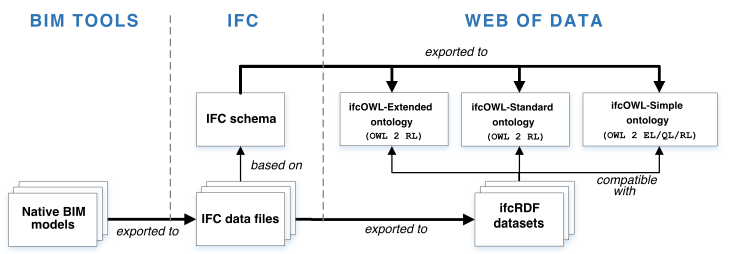
\includegraphics[angle=0,width=1.0\textwidth]{images/ifcOWL-multilayers.png}
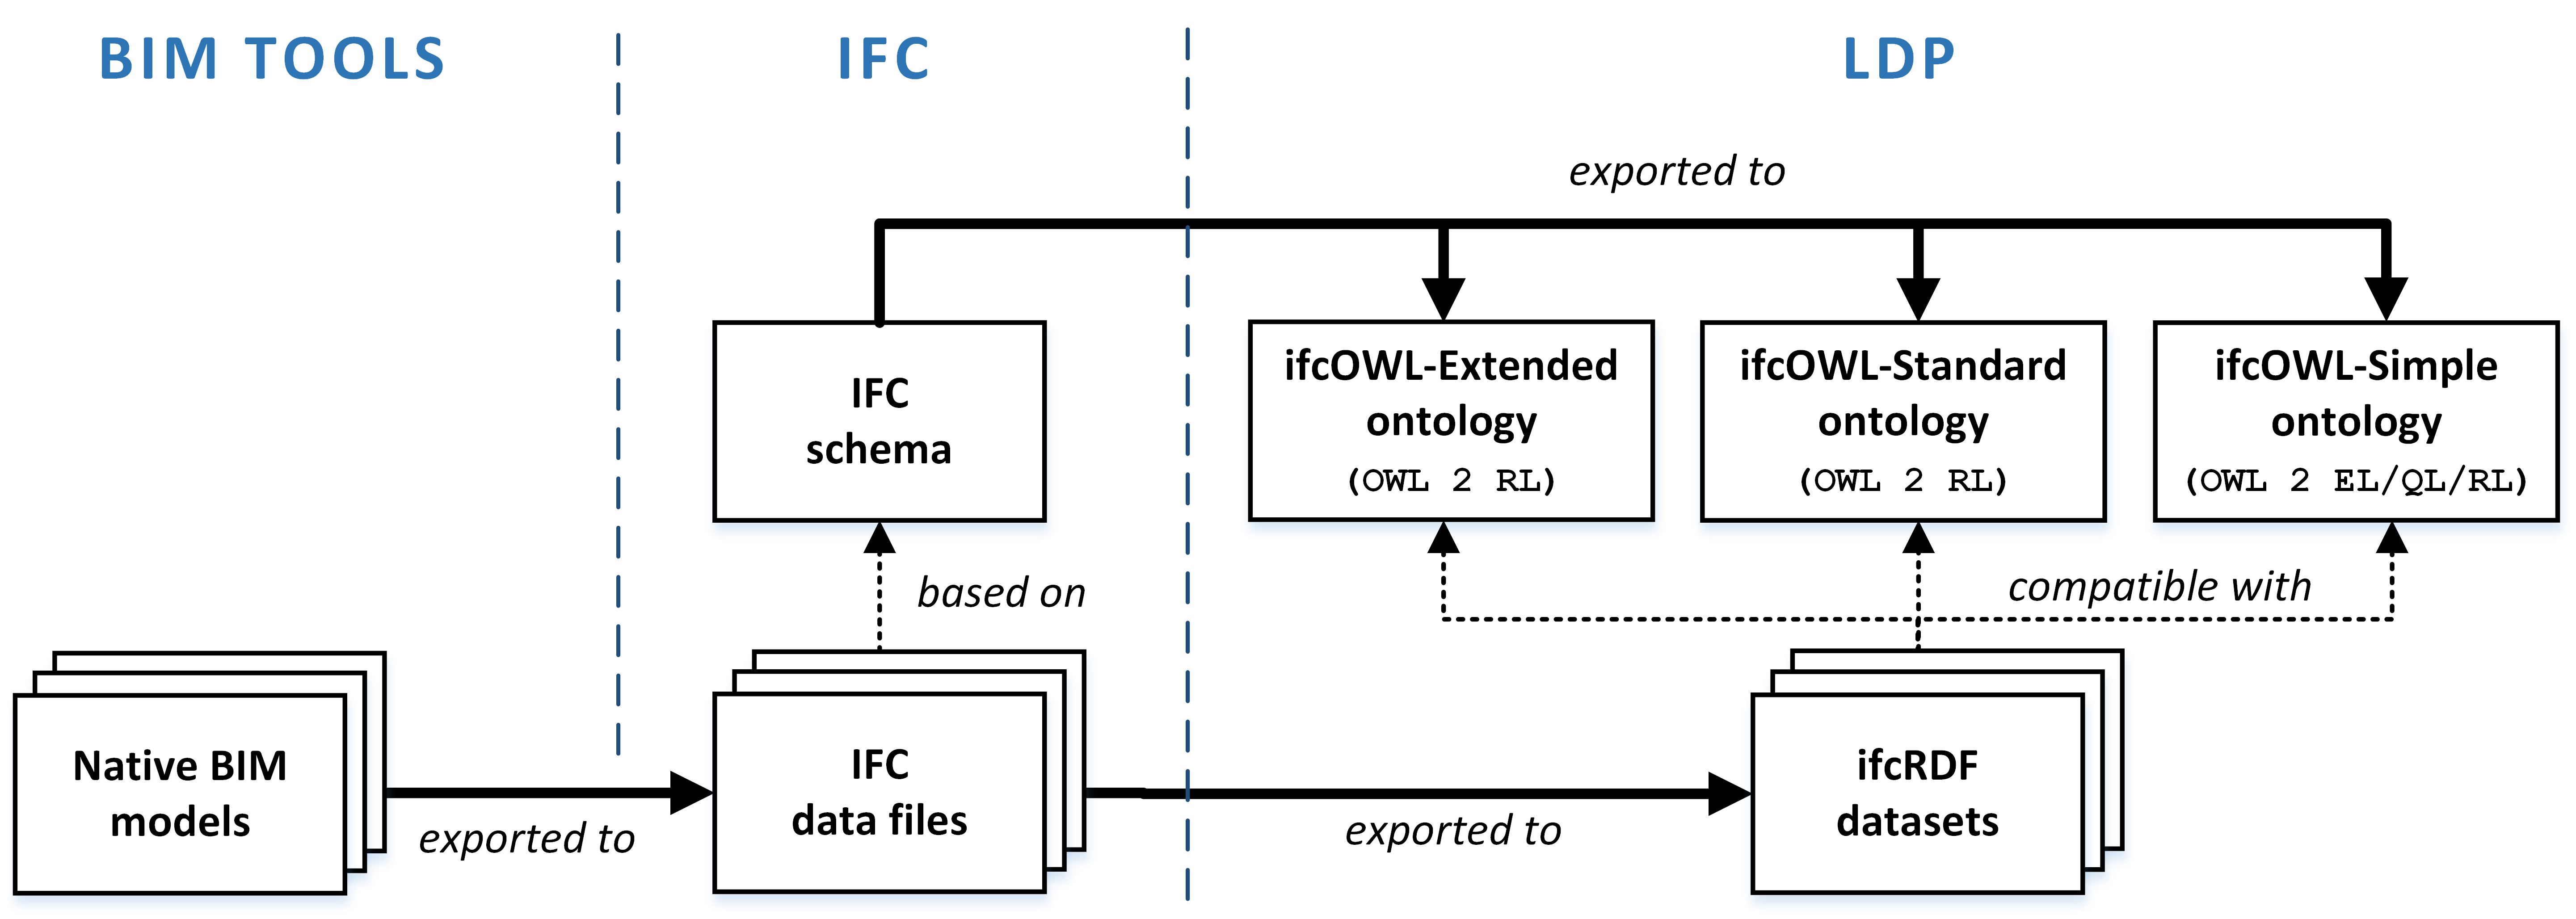
\includegraphics{images/ifcOWL-multilayers-6.png}
%\caption{Multiple layers of \ifcowl{} ontology}
\caption{Producing IFC ontologies and datasets for use in Linked Data Platform}
\label{fig:ifcOWL-layers}
\end{figure}

The conversion of IFC files to \ifcrdf{} is straightforward and can be done 
without information loss.
Ideally, there would also be just one \ifcowl{} ontology for each version of the IFC schema. However,
there are possibilities and reasons to convert the IFC schema to OWL in several different ways. Firstly, there is a \emph{mismatch} between the modeling constructs of OWL and 
EXPRESS data definition language \cite{schenck1994information} used to specify the IFC schema. Secondly, a simple version of \ifcowl{} \emph{compatible with
restricted OWL profiles} (OWL 2 EL or QL) \cite{motik2012owl} is useful to support ontology
reasoning or inexact reasoning. Thirdly, for most practical purposes only a subset of ontology
information is required, as no validation or checking of \ifcrdf{} data is needed; it can
be considered \emph{practically valid} w.r.t. the schema, since BIM tools use certified converters. Moreover, icfRDF can sensibly only be used in a
\emph{read-only} fashion, since BIM models will be maintained in the native formats of BIM
tools. In addition, a full conversion of the IFC schema produces a huge ontology, difficult to understand or manipulate.

Consequently, we convert the IFC schema into a \emph{flexible, multilayer \ifcowl{} ontology}
in a way that \emph{\ifcrdf{} is compatible with any of the layers} (Fig. \ref{fig:ifcOWL-layers}). 
New representational constructs are introduced at more comprehensive levels which therefore 
provide increasing detailed type information about \ifcrdf{} data: 

\vspace{0.5\topsep}
\noindent
\begin{scriptsize}
\begin{center}
    \def\arraystretch{1.2}
    \setlength{\tabcolsep}{6pt}
    \begin{tabularx}{0.95\textwidth}{|l|l|X|}
        \hline
            \textbf{Layer} & \textbf{Profile} & \textbf{Included schema information} \\
        \hline
            ifcOWL-Simple & OWL 2 EL or & Schema meta data plus: \\
            & OWL 2 QL or & \ \ - All type definitions and hierarchies \\
            & OWL 2 RL & \ \ - All entity type properties (names, range types) \\
        \hline 
            ifcOWL-Standard & OWL 2 RL & All above plus: \\
            & & \ \ - All entity type keys \\
            & & \ \ - All entity type inverse properties \\
        \hline
            ifcOWL-Extended & OWL 2 RL & All above plus: \\
            & & \ \ - All cardinality constraints \\
        \hline
    \end{tabularx}
\end{center}
\end{scriptsize}

%Since all \ifcrdf{} datasets are compatible with all layers of the \ifcowl{} ontology 
%(Fig. \ref{fig:ifcOWL-layers}), the most appropriate one can be selected based on the requirements of 
%a use case and tools. For instance, many Linked Data applications that need to 
%query entity properties, use the type hierarchy, or convert \ifcrdf{} datasets back to 
%object-oriented data models it is sufficient to use the \name{ifcOWL-Simple} ontology. 
%In case of reasoning about data that includes inverse properties, it is recommended to use 
%\name{ifcOWL-Standard} ontology. If an RDF dataset needs to be modified and data validated 
%using type and cardinality constraints, \name{ifcOWL-Extended} is the correct choice.


From the previous IFC-to-OWL/RDF conversions
\cite{beetz2005ontology,beetz2009ifcowl,pauwels2011interoperability} our approach differs since it
is based on OWL 2 profiles, produces a flexible multilayer ontology, applies other methods of data\-type definitions and is specifically targeted to
real-life Linked Data applications. It uses stable URIs for entities, in contrast to the previous approaches
where the URIs were instable across models versions.

CityGML \cite{kolbe2005citygml} is a surface model for buildings, which can be useful to visitors for 
indoor navigation. IFC contains complementary information about building design, structure, 
and equipment for a wider range of stakeholders and use cases. Moreover, IFC data can be one source 
when generating CityGML models. % GityGML has also been converted into OWL. 

In the rest of this paper we describe the conversions to \ifcowl{} and \ifcrdf{}, present the deployment of ontologies, example datasets and the converter, and finish with summary and future work. 


%%%%%%%%%%%%%%%%%%%%%%%%%%%%%%%%%%%%%%%%%%%%%
% Converting EXPRESS Schemas to OWL
%%%%%%%%%%%%%%%%%%%%%%%%%%%%%%%%%%%%%%%%%%%%%

\section{Generating ifcOWL Ontologies from the IFC Schema}
\label{sec:ifcOWL}
This section describes the derivation of the ifcOWL ontologies from an IFC schema. The schema defines series of datatypes, functions and rules by using EXPRESS data definition language (ISO10303-11 \cite{schenck1994information}).

\subsection{Basic Principles}

The \ifcsimple{} layer has been designed to be compatible with any OWL 2 DL profile (EL, QL or RL) in order to support a maximum variety of reasoners and other Semantic Web tools. The other layers, i.e. \standard{} and \extended{}, are compatible with OWL 2 RL which -- unlike OWL 2 EL or QL -- supports many important representational constructs of EXPRESS, such as enumerations, union classes and anonymous resources \cite{motik2012owl}. All \ifcowl{} layers include all type definitions and hierarchies so that any \ifcrdf{} datasets converted from IFC data files could reuse types without defining new ones.

The function and rule definitions, type constraints and derived attributes specified in the IFC schema after keywords \name{FUNCTION}, \name{RULE}, and \name{WHERE} are not translated into any \ifcowl{} layer either because of their procedural nature, or the complexity of the resulting constraints.

One goal in the conversion is to keep the property names simple and understandable. Therefore, domain and range constraints (specified by \name{rdfs:domain} and \name{rdfs:range}) are not included in \ifcowl{}. Firstly, there is no need to verify types or to infer types based on properties of \ifcowl{}. Secondly, while in the IFC schema the same property name can appear in multiple different classes, in RDF, property names are \emph{global} and the basic facilities given by domains and ranges do not provide any direct way to indicate that properties are \emph{local} to a class \cite{world2014rdf}. 
%Finally, direct support for such declarations is provided by OWL constructs, e.g. \name{owl:\-onProperty}.

All constructs related to EXPRESS, STEP or IFC specifications belong to separate namespaces shown below with prefixes \name{expr:}, \name{step:} and \name{ifc:} accordingly (\name{IFCxxx} should be replaced by the name of an IFC version, e.g. \name{IFC4\_ADD1}):

%\begin{lstlisting}[caption={Namespace definitions},label=lst:ifcOWL-namespaces]
\begin{lstlisting}
@prefix expr: <http://drumbeat.cs.hut.fi/owl/EXPRESS#>
@prefix step: <http://drumbeat.cs.hut.fi/owl/STEP#>
@prefix ifc:  <http://drumbeat.cs.hut.fi/owl/IFCxxx#>
\end{lstlisting}



%%%%%%%%%%%%%%%%%%%%%%%%%%%%%%%%%%%%%
% Components of an EXPRESS schema
%%%%%%%%%%%%%%%%%%%%%%%%%%%%%%%%%%%%%

\subsection{Datatype Declarations}
\label{subsec:ifcOWL-types}

An EXPRESS schema includes six groups of data\-types, namely: \emph{simple}, \emph{entity}, \emph{enumeration}, \emph{defined}, \emph{select}, and \emph{aggregation} data\-types.


%%%%%%%%%%%%%%%%%%%%%%%%%%%%%%%%%%%%%
% Simple Datatype Declarations
%%%%%%%%%%%%%%%%%%%%%%%%%%%%%%%%%%%%%

\subsubsection{Simple Datatypes} built in EXPRESS are: \name{STRING}, \name{BI\-NA\-RY}, \name{IN\-TE\-GER}, \name{REAL}, \name{NUM\-BER}, \name{BOO\-LEAN}, and \name{LO\-GI\-CAL}. Any simple data\-type, except \name{BOOLEAN} and \name{LOGICAL}, should be declared in \ifcowl{} as \name{owl:sameAs} of its most similar XSD data\-type among the data\-types that are supported by all OWL 2 profiles \cite{motik2012owl} and preferred in Linked Data Platform \cite{ldp-best-practices}:

% \begin{lstlisting}[caption={Simple data types}, label=lst:ifcOWL-simple-types]
\begin{lstlisting}
expr:STRING, ifc:IfcGlobalUniqueId owl:sameAs xsd:string .
expr:BINARY owl:sameAs xsd:hexBinary .
expr:INTEGER owl:sameAs xsd:integer .
expr:REAL, expr:NUMBER owl:sameAs xsd:double .
\end{lstlisting}

Type \name{LOGICAL} -- with its three possible values \name{TRUE}, \name{FALSE} and \name{UNKNOWN} -- is considered as an enumeration data\-type. The same to \name{BOOLEAN} because OWL 2 EL and QL do not support data\-type \name{xsd:boolean} \cite{motik2012owl}.

XSD type \name{xsd:double} is closer to \name{REAL} than \name{xsd:decimal} as it is an IEEE 64-bit floating-point data\-type and supports scientific notation. Whenever a simple data\-type of EXPRESS is needed, its XSD equivalent type should be used directly.
% When it is needed to refer to an EXPRESS simple data\-type, we recommend to use its XSD equivalent type directly.

Types \name{STRING} and \name{BINARY} data\-types may be specified with a size parameter: \name{STRING(\emph{max\-Length\-In\-Bytes})} or \name{BINARY(\emph{size\-In\-Bits})}. It should be ignored in the \simple{} and \standard{} layers, and must be declared in the \extended{} layer:

% \begin{lstlisting}[caption={Size constraint of simple datatypes},label=lst:ifcOWL-simple-types-with-size]
\begin{lstlisting}
# only for the Simple, Standard layers
  expr:STRING22 owl:sameAs xsd:string .
# only for the Extended layer
  expr:STRING22 owl:equivalentClass [ a rdfs:Datatype ;
    owl:onDatatype xsd:string; owl:withRestrictions ( [ xsd:length 22 ] ) ] .
\end{lstlisting}

%%%%%%%%%%%%%%%%%%%%%%%%%%%%%%%%%%%%%
% Enumeration Datatype Declarations
%%%%%%%%%%%%%%%%%%%%%%%%%%%%%%%%%%%%%

\subsubsection{Enumeration Datatypes} represent fixed sets of possible string values. Each enumeration data\-type should be defined in \ifcowl{} as a \emph{subclass}\footnote{Any class that is a subclass of another one hereinafter is an \name{owl:Class}.} of \name{expr:\-Enum\-Class}. Enumeration values are defined as \emph{named individuals} of the enumeration class, but in different ways, according to the layer, since enumerations with more than one individual or literal are not supported in OWL 2 EL or QL:

% \begin{lstlisting}[caption={Enumeration data\-types}, label=lst:ifcOWL-enum-types]
\begin{lstlisting}
# only for the Simple layer
  ifc:IfcAssemblyPlaceEnum a owl:Class ; rdfs:subclassOf expr:EnumClass .
  ifc:SITE, ifc:FACTORY, ifc:NOTDEFINED a ifc:IfcAddressTypeEnum .
# only for the Standard, Extended layers
  ifc:IfcAssemblyPlaceEnum a owl:Class ; rdfs:subclassOf expr:EnumClass ;
     owl:oneOf ( ifc:SITE ifc:FACTORY ifc:NOTDEFINED ) .
\end{lstlisting}

The enumeration values are not defined as literals because enumerations of literals are not supported by OWL 2 RL. The fact that some values -- for instance, \name{ifc:NOT\-DE\-FI\-NED} -- belong to different enumeration data\-types should not cause any problems as an enumeration value can be assigned only to an entity attribute with known enumeration data\-type.

As mentioned above, simple data\-types \name{BOOLEAN} and \name{LOGICAL} are considered as enumerations. However, they and their values should be defined in the EXPRESS-related namespace, e.g. \name{expr:LOGICAL}, \name{expr:TRUE}, \name{expr:UNKNOWN}, etc.


%%%%%%%%%%%%%%%%%%%%%%%%%%%%%%%%%%%%%
% Select Datatype Declarations
%%%%%%%%%%%%%%%%%%%%%%%%%%%%%%%%%%%%%

\subsubsection{Select Datatypes} represent unions of other data\-types. A particular member of a select data\-type can be either an entity, or a defined, or a select data\-type. For instance, type \name{Ifc\-Trim\-ming\-Se\-lect} is an union of entity data\-type \name{Ifc\-Car\-te\-sian\-Point} and defined data\-type \name{Ifc\-Pa\-ra\-me\-ter\-Va\-lue}. A select data\-type is converted into a subclass of \name{expr:\-Select\-Class}. Its particular data\-types are defined as subclasses of the select class, but in different ways, depended on the layer, since property \name{owl:unionOf} is not supported in OWL 2 EL and OWL 2 QL \cite{motik2012owl}:

%\begin{lstlisting}[caption={Select data\-types}, label=lst:ifcOWL-select-types]
\begin{lstlisting}
# only for the Simple layer
  ifc:IfcTrimmingSelect a owl:Class ; rdfs:subclassOf expr:SelectClass .
  ifc:IfcCartesianPoint, ifc:IfcParameterValue
        rdfs:subclassOf ifc:IfcTrimmingSelect .
# only for the Standard, Extended layers
  ifc:IfcTrimmingSelect a owl:Class ; rdfs:subclassOf expr:SelectClass ;
        owl:unionOf ( ifc:IfcCartesianPoint ifc:IfcParameterValue ) ] .
\end{lstlisting}



%%%%%%%%%%%%%%%%%%%%%%%%%%%%%%%%%%%%%
% Defined Datatype Declarations
%%%%%%%%%%%%%%%%%%%%%%%%%%%%%%%%%%%%%

\subsubsection{Defined (Declared, Named) Datatypes} are usually specified as equivalent sets or subsets of simple data\-types or other defined data\-types. For instance, \name{Ifc\-Length\-Mea\-sure} is equal to \name{REAL}, while \name{Ifc\-Po\-si\-ti\-ve\-Length\-Mea\-su\-re} is a subset of \name{Ifc\-Length\-Mea\-sure}, specified by some constraint rule.

A defined data\-type must not be converted into a \name{rdfs:Datatype} even if it is equivalent to a simple data\-type. Let us suppose, there is an attribute with a select type \name{IfcMeasureValue} and it has a \name{xsd:double} value, then it is hard to say whether this is a \name{IfcLengthMeasure} value, a \name{IfcMassMeasure} value, or something else. Furthermore, it is not allowed to use a \name{rdfs:Datatype} as a member class of a select class like \name{ifc:ifcMeasureValue}. 

Thus, a defined data\-type based on a simple data\-type should be converted into an \name{expr:\-Defined\-Class}' subclass which has only property \name{rdf:value} with range is the base simple data\-type. A defined data\-type based on another defined data\-type should be declared as a subclass of the base defined data\-type, for instance:

%\begin{lstlisting}[caption={Defined data\-types}, label=lst:ifcOWL-defined-types]
\begin{lstlisting}
ifc:IfcLengthMeasure a owl:Class ; rdfs:subClassOf expr:DefinedClass ;
    # only for the Standard, Extended layers
    rdfs:subClassOf [ a owl:Restriction; owl:onProperty rdf:value;
                      owl:allValuesFrom xsd:double ] .
ifc:IfcPositiveLengthMeasure rdfs:subClassOf ifc:IfcLengthMeasure .
\end{lstlisting}

In IFC, type \name{Ifc\-Time\-Stamp} is defined as \name{INTEGER} which represents so-called Unix time value. However, it was decided that these values must be converted to standard datetime values during reading IFC files. Thus, \name{ifc:Ifc\-Time\-Stamp} wraps a \name{xsd:date\-Time} property instead of \name{xsd:integer}.


%%%%%%%%%%%%%%%%%%%%%%%%%%%%%%%%%%%%%
% Aggregated Datatype Declarations
%%%%%%%%%%%%%%%%%%%%%%%%%%%%%%%%%%%%%

\subsubsection{Aggregated Types} may be unordered (\name{SET} and \name{BAG}) or  ordered (\name{LIST} and \name{ARRAY}) collections. %\name{BAG} may contain duplicated values, unlike \name{SET}. 
\name{ARRAY} is specified with start and end indexes while other types are specified with min and max cardinalities.

Any aggregated type in \ifcowl{} is a subclass of \name{expr:SetClass},
\name{expr:ListClass}, \name{expr:ArrayClass} or \name{expr:BagClass}. Their common superclass \name{expr:\-Collec\-tion\-Class} has one \emph{nonfunctional} property \name{expr:slot} with type \name{expr:Slot} and four functional properties: \name{expr:isOrdered}, \name{expr:item\-Type}, \name{expr:\-size}, \name{expr:\-start\-Index}, and \name{expr:\-end\-Index}. Class \name{expr:Slot} has functional properties \name{expr:item}, \name{expr:index}, and optional functional properties \name{expr:previous}, \name{expr:next}. A fragment of the definition of type \name{SET [2:?] OF IfcProfileDef} is shown as follows:

\begin{lstlisting}
# all layers:
 ifc:SET_2_UNLIMITED_OF_IfcProfileDef a owl:Class ;
    rdfs:subClassOf ifc:SET_2_UNLIMITED , ifc:SET_OF_IfcProfileDef .
 ifc:SET_2_UNLIMITED, SET_OF_IfcProfileDef rdfs:subClassOf expr:SetClass .

# only for the Extended layer:
 ifc:SET_2_UNLIMITED rdfs:subClassOf rdfs:subClassOf [ a owl:Restriction ;
    owl:onProperty expr:slot ; owl:minCardinality "2"^^xsd:integer ] .
 ifc:SET_OF_IfcProfileDef rdfs:subClassOf [ a owl:Restriction ;
    owl:onProperty expr:slot ; owl:allValuesFrom ifc:SLOT_OF_IfcProfileDef ].
 ifc:SLOT_OF_IfcProfileDef rdfs:subClassOf [ a owl:Restriction ; owl:onProperty expr:item ; owl:allValuesFrom ifc:IfcProfileDef ] .
\end{lstlisting}



%%%%%%%%%%%%%%%%%%%%%%%%%%%%%%%%%%%%%
% Entity Datatype Declarations
%%%%%%%%%%%%%%%%%%%%%%%%%%%%%%%%%%%%%

\subsubsection{Entity Datatypes} correspond to classes in object-oriented languages. Each type may have one super\-type. Thus, an entity data\-type should be converted into a subclass of its super\-class or of \name{expr:\-Entity\-Class}.

The minimum cardinality of an optional entity property is \name{0}. The maximum cardinality is always \name{1}. If an attribute type is set, list, or array, then a new aggregation data\-type is defined, for example, \name{ifc:\-SET\_\-2\_\-UNLIMITED\_\-IfcProfileDef} was created for property \name{Profiles : SET [2:?] OF IfcProfileDef}. This approach allows to represent all multiple attributes in the same manner and provides possibilities to constrain the cardinalities, even when the minimum cardinality is not \name{0} or \name{1}.


% Below is an example of definition of a type with attributes \name{Profiles : SET [2:?] OF IfcProfileDef} and \name{Label : OPTIONAL IfcLabel}:

%\begin{lstlisting}[caption={Entity data\-types}, label=lst:ifcOWL-defined-types]
\begin{lstlisting}
ifc:IfcCompositeProfileDef a owl:Class ; rdfs:subClassOf ifc:IfcProfileDef ;
  # only for the Standard, Extended layers
    rdfs:subClassOf [ a owl:Restriction; owl:onProperty ifc:profiles;
                      owl:allValuesFrom ifc:SET_2_UNLIMITED_IfcProfileDef ] ;
    rdfs:subClassOf [ a owl:Restriction; owl:onProperty ifc:label;
                      owl:allValuesFrom ifc:Label ] ;
  # only for the Extended layer
    rdfs:subClassOf [ a owl:Restriction; owl:onProperty ifc:profiles;
                      owl:cardinality "1"^^xsd:integer ] ;
    rdfs:subClassOf [ a owl:Restriction; owl:onProperty ifc:label;
                      owl:minCardinality "0"^^xsd:integer ] ;
    rdfs:subClassOf [ a owl:Restriction; owl:onProperty ifc:label;
                      owl:maxCardinality "1"^^xsd:integer ] .
\end{lstlisting}



%%%%%%%%%%%%%%%%%%%%%%%%%%%%%%%%%%%%%
% Generating ifcRDF Datasets From IFC Data
%%%%%%%%%%%%%%%%%%%%%%%%%%%%%%%%%%%%%

\section{Generating ifcRDF Datasets from IFC Data}
\label{sec:ifcRDF}

As mentioned in Sect. \ref{sec:introduction}, IFC data is exchanged in STEP Physical Files (SPF). The IFC-SPF-to-RDF conversion is aimed to produce \ifcrdf{} datasets including \emph{all} information stored in SPFs and compatible with any \ifcowl{} layer.

\subsubsection{Header Section} includes STEP-specific metadata as normal data-section entities. Their types -- \name{FileDescription}, \name{FileName}, and \name{FileSchema} -- are defined in STEP. They are exported as normal entities, but some attributes of them are duplicated as Dublin Core (DC) metadata annotations, for example:

\begin{lstlisting}
<http://example.org>  a void:DataSet ;
    dcterms:created "2015-02-19T13:22:15Z"^^xsd:dateTime ;
    dcterms:creator "John Smith"^^xsd:string .
    step:fileName  [ a step:FileName ;
        step:author "John Smith"^^xsd:string ;
        step:originating_system "Tekla Structures 20.1"^^xsd:string ; ] ;
        step:time_stamp "2015-02-19T13:22:15Z"^^xsd:dateTime  ] .
\end{lstlisting}


\subsubsection{Data Section} includes entities, each of which is identified with a line number.
%, an entity data\-type and a list of values. 
All entities of \name{Ifc\-Root}-derived types have a GUID in IFC. They are converted into URI resources with format \name{GUID\_\emph{\textless{}guid\textgreater{}}} where \emph{guid} is in the hexadecimal string representation (not including the character \name{\$}). Regarding to anonymous IFC entities, it can be chosen whether to export them as blank nodes or create them a URI in a format \name{LINE\_\emph{\textless{}lineNumber\textgreater{}}} (in a user defined namespace). Note that line numbers are used only for linking entities inside a SPF, and they are unstable. Naming is required when the dataset is used together with OWL 2 EL/QL as these profiles do not allow anonymous individuals. Below is an example of IFC data exported to an RDF dataset compatible with OWL 2 RL:

\begin{lstlisting}
:GUID_1916794F-5605-4499-9AB0-F155DE8D3B6C     # entity as an URI
    a            ifc:IfcPropertySet ;          # entity type
    ifc:globalId [ a ifc:IfcGloballyUniqueId ; # property with defined type
                   rdf:value "0P5dbFLWL4cPgmyLNUZJji"^^xsd:string ] ;
    ifc:hasProperties  _:b11 .                 # property w/ aggregated type
_:b11 a ifc:SET_1_UNLIMITED_OF_IfcProperty ;
    expr:size "3"^^xsd:integer ;
    expr:itemType ifc:IfcProperty ;
    expr:slot _:b12, _:b13, _:b14 .
_:b12 a ifc:SLOT_OF_IfcProperty ;
    expr:item [ a ifc:IfcPropertySingleValue ;  # entity as a blank node
                ifc:name "initial_GUID"^^xsd:string ;
                ifc:nominalValue  _:b15 ] .
\end{lstlisting}


%Data\-type of an attribute value is declared obviously only if the attribute has a select data\-type and the value has a defined data\-type. 

\section{Implementation and Deployment}
\label{sec:deployment}

The algorithm of generating \ifcowl{} ontologies and \ifcrdf{} datasets, including the principles described in Sect. \ref{sec:ifcOWL}-\ref{sec:ifcRDF}, are implemented in our Java program, namely \textbf{IFC2LD converter}. One can use its command-line interface, web interface or application programming interface for converting any IFC schema or data file into \ifcowl{} or \ifcrdf{}. By changing the configuration file, one can also force the converter to adapt various OWL profiles starting from OWL Lite.

The \textbf{IFC2LD converter}, \ifcowl{} ontologies including different layers for different IFC schema versions, and some sample \ifcrdf{} datasets (together with the original IFC files) are available on the Internet (Table \ref{tab:ifc2ld-web}).

\begin{table}
    \caption{Contents of ifcOWL layers}
    \label{tab:ifc2ld-web}
    \centering
    \scriptsize
    \def\arraystretch{1.2}          % vertical space
    \setlength{\tabcolsep}{6pt}     % horizontal space
    \begin{tabularx}{0.90\textwidth}{|l|X|}
        \hline
        Ontologies: & \texttt{http://drumbeat.cs.hut.fi/owl/} \\
        \hline
        Example files & \\
        - IFC data: & \texttt{http://drumbeat.cs.hut.fi/ifc/} \\
        - RDF datasets: & \texttt{http://drumbeat.cs.hut.fi/rdf/} \\
        \hline
        IFC2LD Converter & \\
        - online service: & \texttt{http://drumbeat.cs.hut.fi/home/} \\
        - download binary: & \texttt{http://drumbeat.cs.hut.fi/ifc2ld/} \\
        % - source code: & \texttt{https://github.com/Web-of-Building-Data/Ifc2Rdf} \\
        \hline
    \end{tabularx}
\end{table}

\section{Summary and future works}
\label{sec:summary}

In this paper, we proposed a new approach and principles of creating \ifcowl{}, a multilayer ontology of building designs based on the widely adopted IFC standard. The ontology is 
derived from the IFC schema with the \ifcld{} converter that can also produce RDF datasets from IFC files. 

The \ifcowl{} ontologies and \ifcrdf{} datasets are currently used in a variety of Linked-Data-oriented use cases \cite{torma2013semantic} which are developed in the DRUMBEAT project. We are exploring the possibilities to use the \ifcld{} converter in the terms of generation of metadata for linksets between \ifcrdf{} datasets.




% According to LNCS manual, the Acknowledgements section must be declared by using \subsubsection{}

\subsubsection{Acknowledgements.} This work has been carried out at Aalto University in research projects DRUM (RYM/PRE 2010-2014) and DRUMBEAT (2014-2017), funded by Tekes, Aalto University, and the participating companies. 

%%
% ---- Bibliography ----
%


\begin{thebibliography}{}

\bibitem{datapic:xsd}
XML Schema 1.1, Datypic, http://www.datypic.com/sc/xsd11/ss.html

\bibitem{noauthor:ifc-guide}
The EXPRESS Definition Language for IFC Development, Stanford University documentation,
"http://web.stanford.edu/group/narratives/classes/08-09/CEE215/ReferenceLibrary/Industry Foundation Classes (IFC)/IFC General/The\_EXPRESS\_Definition\_Language\_for\_IFC\_Development.pdf"

\bibitem{w3c:ldp-best-practices}
Cody Burleson; Miguel Esteban Gutiérrez; Nandana Mihindukulasooriya. LDP Best Practices and Guidelines. W3C Working Draft. URL: http://www.w3.org/2012/ldp/hg/ldp-bp/ldp-bp.html

\bibitem{w3c:owl2-profiles}
World Wide Web Consortium. OWL 2 Web Ontology Language: Profiles (Second Edition), ed. Boris Motik et al. W3C Recommendation, 11 December 2012, http://www.w3.org/TR/2012/REC-owl2-profiles-20121211/. Latest version available at http://www.w3.org/TR/owl2-profiles/

\bibitem{w3c:xsd}
World Wide Web Consortium. W3C XML Schema Definition Language (XSD) 1.1 Part 2: Structures, ed. David Peterson et al. W3C Working Draft 3 December 2009. Available at: http://www.w3.org/TR/xmlschema11-2/

\bibitem{wiki:express}
EXPRESS (data modeling language), Wikipedia, http://en.wikipedia.org/wiki/EXPRESS\_(data\_modeling\_language)

\bibitem{w3c:owl2-syntax}
World Wide Web Consortium. OWL 2 Web Ontology Language 
Structural Specification and Functional-Style Syntax (Second Edition), ed. Boris Motik et al. W3C Recommendation, 11 December 2012, http://www.w3.org/TR/2012/REC-owl2-syntax-20121211/. Latest version available at http://www.w3.org/TR/owl2-syntax/

\bibitem{w3c:xmlschema11-2}
World Wide Web Consortium. W3C XML Schema Definition Language (XSD) 1.1 Part 2: Datatypes, ed. David Peterson et al. W3C Recommendation, 5 April 2012, http://www.w3.org/TR/2012/REC-xmlschema11-2-20120405#partial-implementation/, Section 5.4. Latest version available at http://www.w3.org/TR/xmlschema11-2/#partial-implementation

\bibitem{w3c:owl-guide}
World Wide Web Consortium. OWL Web Ontology Language Guide, ed. Michael K. Smith et al. W3C Recommendation, 10 February 2004, http://www.w3.org/TR/owl-guide/

\bibitem{w3c:rdf-schema}
World Wide Web Consortium. RDF Schema 1.1, ed. Dan Brickley et al. W3C Recommendation, 25 February 2014, http://www.w3.org/TR/rdf-schema

\end{thebibliography}


% \bibliographystyle{splncs03}
\bibliographystyle{splncs}
\bibliography{article.bib}

% \printbibliography{}


\clearpage
\addtocmark[2]{Author Index} % additional numbered TOC entry
\renewcommand{\indexname}{Author Index}
\printindex
\clearpage
\addtocmark[2]{Subject Index} % additional numbered TOC entry
\markboth{Subject Index}{Subject Index}
\renewcommand{\indexname}{Subject Index}
% \input{subjidx.ind}
\end{document}
